% RiskShip -- solución con un sistema neuro-difuso (ANFIS), formato IEEE.
% Compilar con pdfLaTeX:
%   cd papers && Rscript -e 'tinytex::pdflatex("riskship_anfis.tex")'
% En Overleaf: subir este archivo y la carpeta figuras/.
%
% Todas las cifras del ANFIS provienen de la ejecución versionada de
% notebooks/anfis_shipment_loss.ipynb (5 semillas, valores por defecto) y de
% README.md ("Sistema neuro-difuso (ANFIS)"); las de la RNA, de README.md
% ("Protocolo experimental y resultados (RNA)") y del informe
% informe/riskship_rna.tex; las del GP, de papers/riskship_gp.tex y
% results/gp_full_v1/. Las figuras se generan con
% python papers/build_anfis_figures.py: la comparación a partir de esas
% tablas, y las demás copiadas de informe/figuras/anfis/, exportadas por el
% notebook. No se editan a mano.
\documentclass[conference]{IEEEtran}

\usepackage[utf8]{inputenc}
\usepackage[T1]{fontenc}
\usepackage[spanish,es-tabla,es-nodecimaldot,es-noshorthands]{babel}
\usepackage{amsmath}
\usepackage{array}
\usepackage{booktabs}
\usepackage{cite}
\usepackage{graphicx}
\usepackage{url}

\graphicspath{{figuras/}}

% Nombres de columnas del conjunto de datos (admite guiones bajos).
\newcommand{\col}[1]{\texttt{\detokenize{#1}}}

\renewcommand{\IEEEkeywordsname}{Palabras clave}

\begin{document}

\title{RiskShip: Priorización Inteligente de Envíos con Riesgo de Falla\\
{\large Solución con un sistema neuro-difuso (ANFIS)}}

\author{\IEEEauthorblockN{Kevin Bueno S. y Lizeth Portela L.}
\IEEEauthorblockA{\textit{Departamento de Ingeniería, Pontificia Universidad Javeriana}\\
Bogotá D.C., Colombia\\
bueno.kevin@javeriana.edu.co, portelali@javeriana.edu.co}}

\maketitle

\begin{abstract}
RiskShip es un agente de priorización que estima el riesgo de pérdida de un
envío en el momento de su creación, antes del despacho, y ordena los casos para
que un equipo con capacidad limitada revise primero los más críticos. Este
artículo presenta la tercera técnica del proyecto: un sistema de inferencia
difusa adaptativo (ANFIS) de tipo Takagi-Sugeno, entrenado por gradiente en
PyTorch sobre el mismo conjunto de datos, las mismas 13 variables, la misma
partición temporal y el mismo protocolo de cinco semillas que la red neuronal
(RNA) de referencia y que el clasificador simbólico evolucionado con
programación genética (GP). Las variables categóricas entran como su tasa de
pérdida suavizada, estimada solo en entrenamiento y fuera de pliegue por
envío; los centros de las reglas se inicializan con \textit{fuzzy c-means} y
el número de reglas (32) se elige únicamente en validación. En el mes de
prueba el ANFIS alcanza un PR-AUC de 0,753~$\pm$~0,001 y un ROC-AUC de
0,823~$\pm$~0,001, frente a 0,750~$\pm$~0,002 y 0,824~$\pm$~0,002 de la RNA
y 0,639~$\pm$~0,034 y 0,773~$\pm$~0,019 del GP sobre el mismo
\textit{holdout}: iguala a la RNA con la menor dispersión entre semillas de
las tres técnicas, entrena en unos 5~s por semilla y expone funciones de
pertenencia y una base de reglas legibles. La importancia por permutación
vuelve a señalar al dominio del producto (caída de PR-AUC de 0,247), lo que
confirma que el artefacto de extracción sospechado condiciona a las tres
técnicas por igual.
\end{abstract}

\begin{IEEEkeywords}
lógica difusa, ANFIS, Takagi-Sugeno, sistemas neuro-difusos, priorización de
riesgo, logística, partición temporal, interpretabilidad
\end{IEEEkeywords}

\section{Introducción}

Las plataformas de comercio electrónico operan redes logísticas en las que un
envío atraviesa centros de \textit{fulfillment}, \textit{cross-docking},
transporte intermedio y última milla. La capacidad humana de monitoreo es
limitada, de modo que el valor de un modelo no está solo en clasificar bien,
sino en concentrar la atención en la fracción de casos con mayor riesgo. En la
literatura, el riesgo en cadenas de suministro se ha abordado con redes
neuronales~\cite{bortolini,ye}, con métodos evolutivos~\cite{nezamoddini},
con mecanismos de votación~\cite{ifac2022} y, de forma recurrente, con lógica
difusa~\cite{gajovic,aqlan}, por su capacidad de representar juicios
graduales (``un envío pesado'', ``una instalación con historial malo'') en
lugar de umbrales duros. La Sección~\ref{sec:estado} amplía esta revisión
hacia los sistemas neuro-difusos, la codificación de categóricas y la
evaluación bajo desbalance.

RiskShip formula el problema como una clasificación binaria (el envío se
pierde o no) resuelta a través de un puntaje continuo de riesgo que ordena los
casos. La primera entrega del proyecto resolvió esa tarea con redes
neuronales~\cite{informe_rna} y la segunda con programación
genética~\cite{paper_gp}. Este artículo presenta la tercera técnica: un
sistema de inferencia difusa adaptativo (ANFIS)~\cite{jang} de tipo
Takagi-Sugeno~\cite{takagi}. Un ANFIS es a la vez un sistema de reglas
difusas y una red: cada regla tiene antecedentes gaussianos cuyos centros y
anchos se aprenden por gradiente, y un consecuente lineal que propone un
puntaje. A diferencia de la RNA, sus parámetros tienen un significado directo
(el valor típico de cada variable para cada regla y cuánto tolera la regla
alejarse de él); a diferencia del GP, el ajuste es determinista dada la
semilla y no depende de una búsqueda combinatoria. La pregunta es si esa
representación intermedia conserva la calidad de priorización de la red sin
pagar la brecha que mostró el árbol simbólico.

\textbf{Alcance.} Igual que en las entregas anteriores, la tarea se acota a
predecir la \emph{pérdida} en el \emph{momento de creación} del envío. El
ANFIS se evalúa con el mismo protocolo que la RNA y el GP (misma limpieza,
misma partición temporal, mismo conjunto de prueba, cinco semillas y mismas
métricas) para que la comparación sea directa. Ni la RNA ni el GP se
reentrenaron: sus cifras son las publicadas en el repositorio del proyecto.

\section{Estado del arte}
\label{sec:estado}

\subsection{Sistemas de inferencia difusa y ANFIS}

Los conjuntos difusos de Zadeh~\cite{zadeh} permiten que un valor pertenezca
en grado a una categoría lingüística, y un sistema de inferencia difusa
combina reglas ``SI--ENTONCES'' sobre esas categorías. Takagi y
Sugeno~\cite{takagi} propusieron reglas cuyo consecuente es una función
lineal de las entradas, lo que convierte el sistema en una mezcla de modelos
locales ponderada por el grado de activación de cada regla. Jang~\cite{jang}
mostró que un sistema Takagi-Sugeno puede escribirse como una red adaptativa
de cinco capas (fuzzificación, activación, normalización, consecuentes y
agregación) y entrenarse con un procedimiento híbrido: mínimos cuadrados para
los consecuentes y descenso de gradiente para los antecedentes. Esa
arquitectura, ANFIS, es la que adopta RiskShip, con dos adaptaciones
habituales en clasificación: la salida pasa por una sigmoide y se entrena con
entropía cruzada, de modo que los mínimos cuadrados ya no tienen solución
cerrada y todos los parámetros se ajustan por gradiente con
Adam~\cite{adam}; y la activación se calcula en logaritmos para que el
producto de trece pertenencias no se anule numéricamente.

\subsection{Diseño de reglas a partir de datos e interpretabilidad}

Guillaume~\cite{guillaume} revisa los métodos para inducir sistemas difusos a
partir de datos y advierte que la precisión suele obtenerse a costa de la
legibilidad: particiones que no se corresponden con etiquetas lingüísticas,
reglas redundantes o que nunca se activan. Dos prácticas de esa revisión
guían el diseño de RiskShip. La primera es inicializar las reglas con un
agrupamiento difuso, el \textit{fuzzy c-means} de Bezdek~\cite{bezdek}, de
modo que cada regla nazca cubriendo una región real del espacio de entrada en
lugar de una posición aleatoria que quizá nunca se active. La segunda es
reportar la base de reglas resultante con etiquetas lingüísticas y con la
cobertura efectiva de cada regla, para que la interpretabilidad se evalúe y
no se suponga. Fernández \textit{et al.}~\cite{fernandez} estudian los
clasificadores difusos lingüísticos con clases desbalanceadas y muestran que
la granularidad de la partición y el tratamiento del desbalance determinan su
comportamiento; aquí el desbalance se trata con una métrica de orden en la
selección y la parada temprana, no con remuestreo. Rudin~\cite{rudin}
sostiene que en decisiones de alto impacto debe preferirse un modelo
interpretable a la explicación a posteriori de una caja negra; el ANFIS ocupa
una posición intermedia, y este artículo la caracteriza en lugar de
reclamarla.

\subsection{Variables categóricas de alta cardinalidad}

Un sistema difuso solo opera sobre entradas numéricas. Micci-Barreca~\cite{micci}
propuso codificar una categoría por su tasa objetivo suavizada hacia el previo
global, con un peso que protege a las categorías raras de memorizar sus pocos
casos. Prokhorenkova \textit{et al.}~\cite{catboost} señalan el sesgo de esa
codificación cuando se calcula con las mismas filas que luego se entrenan (la
etiqueta de cada fila se filtra a su propia variable) y lo resuelven con
estadísticas ordenadas, calculadas sin la fila en cuestión. RiskShip aplica
la codificación de Micci-Barreca con la corrección de CatBoost en su forma
fuera de pliegue, con pliegues por envío porque los artículos de un mismo
envío comparten etiqueta y categorías.

\subsection{Aprendizaje automático en riesgo logístico}

Además de los trabajos citados en la introducción, la predicción de fallas en
la última milla se ha abordado con aprendizaje supervisado: De Leeuw
\textit{et al.}~\cite{deleeuw} predicen la pérdida de paquetes sobre un año
de envíos y recurren a explicabilidad a posteriori; Zhang
\textit{et al.}~\cite{zhang2026} proponen una red tabular para el retraso en
comercio electrónico. La lógica difusa en riesgo logístico se ha usado sobre
todo con reglas escritas por expertos~\cite{gajovic,aqlan}; no se encontró un
trabajo que aprenda un sistema difuso a partir de datos para la pérdida de
envíos bajo un protocolo temporal, que es la aportación de este artículo.

\subsection{Evaluación bajo desbalance y fuga de información}

Davis y Goadrich~\cite{davis} demuestran que una curva domina en el espacio
ROC si y solo si domina en el espacio precisión-exhaustividad, y que este
último es más informativo cuando la clase positiva es minoritaria; Saito y
Rehmsmeier~\cite{saito} lo confirman empíricamente. Kaufman
\textit{et al.}~\cite{kaufman} formalizan la fuga de información como el uso
de datos que no están legítimamente disponibles en el momento de la
predicción. Ambas líneas sustentan el protocolo compartido de RiskShip: la
precisión promedio como métrica principal y criterio de parada temprana, la
partición temporal por mes, la codificación de categóricas calculada solo con
entrenamiento y la exclusión de las columnas de la Tabla~\ref{tab:fuga}.

\section{Motivación y contextualización del problema}

\subsection{Problema de aplicación}

La aplicación considera una operación logística de comercio electrónico. El
equipo adoptó una prevalencia operacional de referencia del 0,1\,\% en la
primera entrega~\cite{informe_rna}; es una estimación de contexto, no una
estadística medida en este conjunto. Cada pérdida implica reembolso,
reposición y deterioro de la confianza del comprador. El equipo que puede
intervenir (verificar el empaque, reforzar el seguimiento, cambiar la ruta)
tiene una capacidad fija, muy inferior al volumen diario. La pregunta
operativa no es ``¿se perderá este envío?'' sino ``¿cuáles de los envíos
creados hoy merecen la atención disponible?''. Un puntaje de riesgo que
ordene los envíos la resuelve directamente.

Los datos disponibles son una muestra de casos y controles: se conservaron las
pérdidas y solo una fracción de los envíos sin pérdida, de modo que la tasa de
positivos de la muestra (24,3\,\% en bruto, 37\,\% tras la limpieza) no es la
real. Esto condiciona qué métricas se trasladan a la operación
(Sección~\ref{sec:alcance}).

\subsection{Pregunta y objetivo}

Para el módulo difuso la pregunta se concreta así: \emph{¿puede un sistema
neuro-difuso aprendido de los datos priorizar las pérdidas al nivel de la red
neuronal y, al mismo tiempo, ofrecer una representación legible por reglas?}
El objetivo es doble: (i) medir el desempeño de priorización del ANFIS sobre
el mismo \textit{holdout} temporal que la RNA y el GP, con cinco semillas y
selección solo por validación; y (ii) caracterizar el modelo obtenido en
número de reglas, cobertura y legibilidad de cada una, costo computacional y
dependencia de la variable de dominio del producto, sobre la que pesa una
sospecha de artefacto de extracción~\cite{informe_rna,paper_gp}.

\section{Descripción de la tarea}

\subsection{Especificación}

\textbf{Entrada.} Un registro de artículo de envío con las 13 variables
conocidas en la creación: seis categóricas (\col{PICKING_TYPE},
\col{SHP_LG_FACILITY_ID}, \col{DOM_DOMAIN_ID}, \col{ORD_CATEGORY_NAME_L1},
\col{BRAND_NAME}, \col{TIPO_BULKY}), seis numéricas (\col{PESO_TOTAL_KG},
\col{DIM_MAX_CM}, \col{VALOR_TOTAL_USD}, \col{CANTIDAD_ITEMS},
\col{RATIO_SVC_MES_ANTERIOR}, \col{ES_BULKY}) y el día de la semana derivado
de \col{date_status_0}. Ninguna fecha absoluta es admisible: permitiría
reaprender el sesgo de madurez de la etiqueta descrito abajo.

\textbf{Salida.} Un puntaje en $[0,1]$, la sigmoide del logit agregado del
sistema, que ordena los artículos; y una decisión binaria con umbral 0,5, el
mismo punto operativo de la RNA. El puntaje está en la escala de la muestra y
no es una probabilidad de producción.

\textbf{Exclusiones por fuga de información.} El análisis de la primera
entrega~\cite{informe_rna} identificó columnas que no existen al crear el
envío o que codifican la etiqueta por la forma en que se extrajeron las
clases; el ANFIS hereda íntegramente esas exclusiones
(Tabla~\ref{tab:fuga}). Además se eliminan las filas con nulos en peso,
dimensión, valor, cantidad o fecha de inicio (casi todas perdidas, un
artefacto de extracción) y los meses recientes cuya etiqueta aún no ha
madurado: se conservan los meses con ambas clases presentes y se descartan
los finales cuya tasa de pérdida es inferior a la mitad de la mediana
mensual. La función de limpieza del \textit{notebook} del ANFIS es una copia
literal de la del \textit{notebook} de la RNA, de modo que los dos modelos
ven exactamente las mismas filas.

\begin{table}[htbp]
\caption{Fuentes de fuga de información heredadas del protocolo RNA}
\label{tab:fuga}
\centering
\footnotesize
\begin{tabular}{>{\raggedright\arraybackslash}p{0.35\linewidth}>{\raggedright\arraybackslash}p{0.53\linewidth}}
\toprule
\textbf{Fuente} & \textbf{Motivo}\\
\midrule
Causa, clasificación y reembolso de la pérdida (9 columnas) & No nulas en el 100\,\% de las filas perdidas y en el 0\,\% del resto\\
\col{status_0..10},\newline \col{date_status_1..10} & Línea de tiempo posterior a la creación\\
\col{DATEPARAMETER} & Igual al inicio del envío si no se perdió; unos 9 días posterior si se perdió\\
\col{LG_REGION} & La misma instalación recibe nombres de región distintos según la clase\\
\col{SHIPMENT_ID}, \col{ITE_ITEM_ID} & Identificadores, no atributos\\
\bottomrule
\end{tabular}
\end{table}

\subsection{Caracterización como agente racional y SMA}

Con la plantilla PEAS, la \emph{medida de desempeño} de RiskShip es la
fracción de pérdidas reales que caen dentro del grupo revisado dada una
capacidad fija (Recall@$K$), junto con el costo de los falsos positivos; su
\emph{entorno} es el flujo de envíos recién creados, parcialmente observable
(solo los 13 atributos de la especificación son visibles), estocástico y
secuencial; sus \emph{actuadores} son la lista ordenada y la marca de
``revisar'' que recibe el equipo humano, que conserva la decisión final; y sus
\emph{sensores} son los atributos del envío en la creación.

En la arquitectura del proyecto el puntaje no lo produce un único modelo, sino
un conjunto de agentes evaluadores (la RNA, el GP y ahora el ANFIS) que
comparten entrada y contrato de salida, de modo que un coordinador pueda
consultarlos, compararlos o combinarlos, y un agente humano cierre el ciclo
revisando casos y realimentando etiquetas. En ese sistema multiagente (SMA) el
módulo ANFIS es el evaluador por reglas: puede mostrar al revisor qué regla
dominó el puntaje de un envío y en qué términos lingüísticos se describe esa
regla, una justificación distinta de la fórmula del GP y de las importancias
a posteriori de la RNA.

\subsection{Alcance y restricciones}
\label{sec:alcance}

Las restricciones se mantienen iguales a las de las entregas anteriores.
(a)~\textbf{Nivel de artículo:} una fila es un artículo, no un envío (cerca de
246\,000 envíos en 262\,317 filas); las métricas son por artículo y ningún
\col{SHIPMENT_ID} aparece en dos particiones. (b)~\textbf{Casos y
controles:} la exhaustividad, la tasa de falsos positivos y el ROC-AUC no
dependen directamente de la prevalencia, pero su traslado a la operación
requiere que el muestreo preserve las distribuciones de puntajes dentro de
cada clase, supuesto que los artefactos de extracción ponen en duda. La
precisión, el PR-AUC, Recall@$K$ y Precision@$K$ dependen de la prevalencia
y describen solo la calidad del orden dentro de la muestra; la mejora sobre
el azar nunca es comparable con producción, pues su techo es $1/\pi$, cerca
de 3 en la muestra y cerca de 1\,000 en producción. (c)~\textbf{Puntaje sin
calibrar:} la sigmoide acota el puntaje a $[0,1]$ pero no lo convierte en una
probabilidad de producción; el umbral 0,5 es el de la muestra.
(d)~\textbf{\textit{Holdout} conocido:} el mes de prueba ya se había
observado al evaluar la RNA y el GP; esta es una comparación con
\textit{holdout} fijo, no una validación ciega nueva. (e)~\textbf{Regla de
madurez retrospectiva:} la selección de meses usa las etiquetas del conjunto
completo; define la cohorte, no es una política operativa validada.

\section{Solución con un sistema neuro-difuso}

\subsection{Codificación de las variables}
\label{sec:codificacion}

Una función de pertenencia gaussiana necesita una entrada numérica sobre la
que medir cercanía. Las seis categóricas y el día de la semana se convierten
en su tasa de pérdida suavizada~\cite{micci}:
\begin{equation}
\tilde{x}_c = \frac{n_c\,\bar{y}_c + m\,\bar{y}}{n_c + m},
\label{eq:te}
\end{equation}
donde $n_c$ y $\bar{y}_c$ son la cantidad de filas y la tasa de pérdida de
la categoría $c$ en entrenamiento, $\bar{y}$ la tasa global de entrenamiento
y $m = 20$ el peso del previo. Las categorías no vistas en entrenamiento
reciben $\bar{y}$. Dos fugas se cierran de forma explícita. Hacia validación
y prueba, las tasas se estiman solo con entrenamiento. Dentro del
entrenamiento, cada fila se codifica \emph{fuera de pliegue}: con cinco
pliegues agrupados por \col{SHIPMENT_ID}, la tasa que ve una fila se calcula
con los otros cuatro pliegues, de modo que ni su propia etiqueta ni la de los
artículos de su mismo envío entran en su variable~\cite{catboost}.

Las numéricas de cola larga (\col{PESO_TOTAL_KG}, \col{DIM_MAX_CM},
\col{VALOR_TOTAL_USD}, \col{CANTIDAD_ITEMS}) pasan por $\log(1+x)$ para que
una gaussiana pueda cubrirlas sin que unos pocos valores extremos la estiren;
los nulos residuales de las numéricas se rellenan con la mediana de
entrenamiento. Al final las 13 columnas se estandarizan con media y
desviación de entrenamiento. La Tabla~\ref{tab:codificacion} resume la
cardinalidad y el rango de las tasas aprendidas; nótese que el 20,9\,\% de
las filas de prueba trae una marca no vista en entrenamiento y entra con el
previo, mientras que las demás categóricas están cubiertas casi por completo.

\begin{table}[htbp]
\caption{Codificación de las categóricas en entrenamiento}
\label{tab:codificacion}
\centering
\scriptsize
\setlength{\tabcolsep}{3pt}
\begin{tabular}{lrrrr}
\toprule
\textbf{Variable} & \textbf{Categorías} & \textbf{Tasa mín.} & \textbf{Tasa máx.} & \textbf{No vistas$^{a}$}\\
\midrule
\col{PICKING_TYPE} & 4 & 0,031 & 0,398 & 0,0\,\%\\
\col{SHP_LG_FACILITY_ID} & 94 & 0,024 & 0,944 & 0,0\,\%\\
\col{DOM_DOMAIN_ID} & 2\,764 & 0,202 & 0,982 & 0,4\,\%\\
\col{ORD_CATEGORY_NAME_L1} & 61 & 0,059 & 0,591 & 0,0\,\%\\
\col{BRAND_NAME} & 22\,761 & 0,177 & 0,885 & 20,9\,\%\\
\col{TIPO_BULKY} & 3 & 0,348 & 0,391 & 0,0\,\%\\
\col{day_of_week} & 7 & 0,356 & 0,418 & 0,0\,\%\\
\bottomrule
\multicolumn{5}{l}{$^{a}$ Fracción de filas de prueba cuya categoría}\\
\multicolumn{5}{l}{\phantom{$^{a}$ }no aparece en entrenamiento.}\\
\end{tabular}
\end{table}

\subsection{Arquitectura}

Con $R$ reglas sobre $d = 13$ entradas, cada regla $r$ tiene la forma
``SI $x_1$ es $A_{r,1}$ Y \dots{} Y $x_d$ es $A_{r,d}$ ENTONCES
$y_r = \mathbf{a}_r^{\top}\mathbf{x} + b_r$'' y la red la implementa en cinco
capas~\cite{jang}:
\begin{align}
\mu_{r,i}(x_i) &= \exp\!\Big(-\tfrac{1}{2}\big(\tfrac{x_i - c_{r,i}}{\sigma_{r,i}}\big)^{2}\Big),
\label{eq:mf}\\
w_r &= \prod_{i=1}^{d} \mu_{r,i}(x_i),\qquad
\bar{w}_r = \frac{w_r}{\sum_{k=1}^{R} w_k},
\label{eq:firing}\\
z &= \sum_{r=1}^{R} \bar{w}_r\,(\mathbf{a}_r^{\top}\mathbf{x} + b_r),\qquad
\hat{p} = \sigma(z).
\label{eq:out}
\end{align}
La conjunción (\ref{eq:firing}) usa la t-norma producto y se calcula como
$\log w_r = -\tfrac{1}{2}\sum_i ((x_i - c_{r,i})/\sigma_{r,i})^{2}$, con lo
que la normalización es una \textit{softmax} sobre las reglas y el producto
de trece pertenencias pequeñas no se anula. Los anchos se guardan en
logaritmo para que sean siempre positivos. Todos los parámetros (centros,
anchos, pesos y sesgos de los consecuentes, $40R$ en total: 1\,280 con
$R = 32$) se ajustan minimizando la entropía cruzada binaria de $\hat{p}$ con
Adam~\cite{adam} en PyTorch~\cite{pytorch}, tasa de aprendizaje
$5\times10^{-3}$ y lotes de 2\,048 filas. El \textit{notebook} verifica que
$\sum_r \bar{w}_r = 1$ en cada fila.

\subsection{Inicialización}

Con centros al azar, muchas reglas nacen en regiones vacías del espacio de
entrada y nunca se activan. Por eso los centros se inicializan con
\textit{fuzzy c-means}~\cite{bezdek} ($m = 2$, 50 iteraciones) sobre una
muestra de 20\,000 filas de entrenamiento; los anchos, con la dispersión
ponderada de cada grupo (mínimo 0,2 en la escala estandarizada); y el sesgo
$b_r$ de cada consecuente, con el logit de la tasa de pérdida ponderada de su
grupo, de modo que cada regla arranca diciendo algo razonable sobre su
región. Los pesos $\mathbf{a}_r$ parten de cero.

\subsection{Entrenamiento, parada temprana y selección de reglas}

Cada entrenamiento recorre hasta 60 épocas y evalúa la precisión promedio en
validación al final de cada una; se conserva el estado de la mejor época y se
detiene tras ocho épocas sin mejora. El número de reglas es el
hiperparámetro estructural: pocas reglas dan un modelo casi lineal, muchas lo
dejan memorizar. Se entrenó una vez por candidato $R \in \{8, 16, 32, 64\}$
con la semilla base y se eligió el de mayor PR-AUC en validación
(Tabla~\ref{tab:reglas}): 32 reglas, con 0,7655; el conjunto de prueba no
intervino. Después se repitió el entrenamiento con $R = 32$ para las cinco
semillas.

\begin{table}[htbp]
\caption{Selección del número de reglas (semilla 42, solo validación)}
\label{tab:reglas}
\centering
\footnotesize
\begin{tabular}{rrrr}
\toprule
\textbf{Reglas} & \textbf{PR-AUC val.} & \textbf{Mejor época} & \textbf{Tiempo (s)}\\
\midrule
8 & 0,7595 & 56 & 4,1\\
16 & 0,7645 & 31 & 3,1\\
32 & \textbf{0,7655} & 36 & 4,8\\
64 & 0,7634 & 20 & 4,5\\
\bottomrule
\end{tabular}
\end{table}

\section{Validación experimental}

\subsection{Datos y partición}
\label{sec:datos}

Se usa el mismo conjunto unificado de la RNA: 262\,317 filas y 58 columnas,
con la etiqueta binaria \col{is_lost}. Tras los filtros de la Sección~IV
quedan 165\,002 filas de 2025-09 a 2026-03. La partición es temporal
(Tabla~\ref{tab:particion}): los meses más antiguos entrenan y los dos más
recientes validan y prueban. Todas las filas de un envío comparten fecha de
inicio, de modo que ningún envío queda repartido entre particiones; el código
lo verifica en cada ejecución.

\begin{table}[htbp]
\caption{Partición temporal de los datos limpios (idéntica a la de la RNA y el GP)}
\label{tab:particion}
\centering
\footnotesize
\begin{tabular}{lcrrr}
\toprule
\textbf{Partición} & \textbf{Meses} & \textbf{Filas} & \textbf{Envíos} & \textbf{Positivos}\\
\midrule
Entrenamiento & 2025-09 a 2026-01 & 125\,082 & 112\,303 & 39,0\,\%\\
Validación & 2026-02 & 18\,831 & 17\,297 & 31,6\,\%\\
Prueba & 2026-03 & 21\,089 & 19\,506 & 31,2\,\%\\
\bottomrule
\end{tabular}
\end{table}

\subsection{Protocolo}

El protocolo replica el de la RNA: cinco semillas (42 a 46) sobre la misma
partición, donde la semilla cambia solo el entrenamiento (muestra del
\textit{fuzzy c-means}, inicialización y orden de los lotes); media y
desviación estándar muestral ($\mathrm{ddof}=1$) sobre el mes de prueba;
selección del número de reglas únicamente en validación, y análisis
detallado con la semilla de mejor PR-AUC en validación, nunca en prueba. Las
métricas son PR-AUC, ROC-AUC, exhaustividad, precisión, F1 y tasa de falsos
positivos de la clase ``perdido'' en el umbral 0,5, y Recall@$K$ y
Precision@$K$ para $K \in \{1, 5, 10, 20\}$\,\% con el mismo desempate
estable de la RNA. A diferencia del GP, el ANFIS comparte con la RNA el
umbral 0,5 sobre una salida sigmoide, de modo que exhaustividad, precisión y
F1 sí son comparables entre ambos en el mismo punto operativo. Ni la RNA ni
el GP se reentrenaron: sus cifras provienen de los informes
anteriores~\cite{informe_rna,paper_gp}.

\subsection{Reproducibilidad}

El \textit{notebook} ejecutado, con todas las tablas y figuras, está
versionado en el repositorio de RiskShip:
\begin{quote}
\footnotesize
\url{https://github.com/aristotekean/riskship-rna}
\end{quote}
bajo \path{notebooks/anfis_shipment_loss.ipynb}; la versión revisada es el
commit \texttt{2b18f26}. El entorno registrado usa Python 3.12, PyTorch
2.10.0, scikit-learn 1.9.1 y pandas 2.3.3, fijados en \texttt{uv.lock};
PyTorch llega con la pila de AutoGluon de la RNA, así que no se agregó
ninguna dependencia. Con el conjunto de datos original, la ejecución completa
se lanza desde la raíz del repositorio con:

{\footnotesize
\begin{verbatim}
uv run jupyter nbconvert --to notebook \
  --execute --inplace \
  notebooks/anfis_shipment_loss.ipynb
\end{verbatim}
}
Las variables de entorno \texttt{ANFIS\_N\_SEEDS}, \texttt{ANFIS\_MAX\_EPOCHS}
y \texttt{ANFIS\_RULE\_GRID} permiten una prueba de humo, que no es un
resultado reportable. Las figuras de este artículo se reconstruyen con
\texttt{python papers/build\_anfis\_figures.py}, que copia las que exporta el
\textit{notebook} y dibuja la comparación a partir de las tablas publicadas;
no entrena modelos. La ejecución completa tarda menos de un minuto en CPU.

\subsection{Resultados}

\textbf{Por semilla.} La Tabla~\ref{tab:semillas} muestra las cinco corridas
con 32 reglas. El PR-AUC de prueba va de 0,7516 (semilla 44) a 0,7546
(semilla 46), un rango de 0,003; la mejor época oscila entre 26 y 52 y cada
entrenamiento tarda entre 3,6 y 6,3~s. La semilla con mejor validación (44,
PR-AUC 0,7676) resulta ser la de menor PR-AUC en prueba, lo que ilustra por
qué la selección no debe mirar la prueba: con una dispersión de 0,001, el
orden entre semillas en prueba no es informativo.

\begin{table*}[htbp]
\caption{Corridas con 32 reglas: validación, prueba y costo por semilla}
\label{tab:semillas}
\centering
\footnotesize
\setlength{\tabcolsep}{5pt}
\begin{tabular}{lrrrrrrrrrr}
\toprule
& \textbf{PR-AUC} & \multicolumn{7}{c}{\textbf{Prueba}} & \textbf{Mejor} & \textbf{Tiempo}\\
\cmidrule(lr){3-9}
\textbf{Semilla} & \textbf{val.} & \textbf{PR-AUC} & \textbf{ROC-AUC} & \textbf{Exhaust.} & \textbf{Precisión} & \textbf{F1} & \textbf{TFP} & \textbf{Recall@20\,\%} & \textbf{época} & \textbf{(s)}\\
\midrule
42 & 0,7655 & 0,7524 & 0,8237 & 0,5635 & 0,7226 & 0,6332 & 0,0982 & 0,5000 & 36 & 4,7\\
43 & 0,7617 & 0,7536 & 0,8232 & 0,5583 & 0,7283 & 0,6321 & 0,0945 & 0,5032 & 26 & 3,6\\
44 & \textbf{0,7676} & 0,7516 & 0,8220 & 0,5574 & 0,7286 & 0,6316 & 0,0942 & 0,5029 & 52 & 6,3\\
45 & 0,7660 & 0,7520 & 0,8228 & 0,5726 & 0,7140 & 0,6355 & 0,1041 & 0,5024 & 28 & 3,8\\
46 & 0,7639 & 0,7546 & 0,8241 & 0,5567 & 0,7329 & 0,6328 & 0,0920 & 0,5065 & 35 & 4,5\\
\midrule
Media & 0,7649 & 0,7529 & 0,8231 & 0,5617 & 0,7253 & 0,6330 & 0,0966 & 0,5030 & 35,4 & 4,6\\
Desv. est. & 0,0022 & 0,0012 & 0,0008 & 0,0067 & 0,0073 & 0,0015 & 0,0047 & 0,0023 & 10,2 & 1,1\\
\bottomrule
\end{tabular}
\end{table*}

\textbf{Agregado y comparación.} La Tabla~\ref{tab:comparacion} resume las
tres técnicas sobre el mismo mes de prueba. El ANFIS obtiene un PR-AUC de
0,7529~$\pm$~0,0012 y un ROC-AUC de 0,8231~$\pm$~0,0008, frente a
0,7496~$\pm$~0,0020 y 0,8241~$\pm$~0,0020 de la RNA; la diferencia en PR-AUC
(+0,0033) es del orden de la suma de ambas desviaciones y la de ROC-AUC
($-$0,0010) es menor que la desviación de la RNA, de modo que las dos
técnicas empatan en calidad de orden. En el umbral común 0,5 el ANFIS tiene
mayor exhaustividad (0,562 frente a 0,534), menor precisión (0,725 frente a
0,757) y F1 ligeramente mayor (0,633 frente a 0,626), con una tasa de falsos
positivos de 0,097 frente a 0,078: sitúa su punto operativo un poco más
hacia la exhaustividad que la RNA. Frente al GP, el ANFIS está 0,114 por
encima en PR-AUC y 0,050 en ROC-AUC, con una dispersión 28 veces menor. La
referencia de PR-AUC para un orden aleatorio es la tasa de positivos, 0,312.

\begin{table}[htbp]
\caption{Métricas en el conjunto de prueba, media $\pm$ desviación estándar sobre cinco semillas (mismo holdout temporal)}
\label{tab:comparacion}
\centering
\scriptsize
\setlength{\tabcolsep}{2.5pt}
\begin{tabular}{lccc}
\toprule
\textbf{Métrica} & \textbf{ANFIS} & \textbf{RNA}$^{a}$ & \textbf{GP}$^{a}$\\
\midrule
PR-AUC & 0,7529 $\pm$ 0,0012 & 0,7496 $\pm$ 0,0020 & 0,6393 $\pm$ 0,0338\\
ROC-AUC & 0,8231 $\pm$ 0,0008 & 0,8241 $\pm$ 0,0020 & 0,7734 $\pm$ 0,0186\\
Exhaustividad$^{b}$ & 0,5617 $\pm$ 0,0067 & 0,5339 $\pm$ 0,0136 & 0,6732 $\pm$ 0,0408\\
Precisión$^{b}$ & 0,7253 $\pm$ 0,0073 & 0,7568 $\pm$ 0,0157 & 0,5506 $\pm$ 0,0369\\
F1$^{b}$ & 0,6330 $\pm$ 0,0015 & 0,6259 $\pm$ 0,0044 & 0,6039 $\pm$ 0,0129\\
Tasa de falsos positivos$^{b}$ & 0,0966 $\pm$ 0,0047 & 0,0781 $\pm$ 0,0089 & ---\\
\midrule
Recall@1\,\% & 0,0321 $\pm$ 0,0000 & 0,0321 $\pm$ 0,0000 & 0,0270 $\pm$ 0,0034\\
Recall@5\,\% & 0,1601 $\pm$ 0,0000 & 0,1581 $\pm$ 0,0006 & 0,1343 $\pm$ 0,0127\\
Recall@10\,\% & 0,3107 $\pm$ 0,0007 & 0,3019 $\pm$ 0,0020 & 0,2595 $\pm$ 0,0172\\
Recall@20\,\% & 0,5030 $\pm$ 0,0023 & 0,5060 $\pm$ 0,0024 & 0,4450 $\pm$ 0,0199\\
\midrule
Precision@1\,\% & 1,0000 $\pm$ 0,0000 & 1,0000 $\pm$ 0,0000 & 0,8427 $\pm$ 0,1061\\
Precision@5\,\% & 1,0000 $\pm$ 0,0000 & 0,9873 $\pm$ 0,0038 & 0,8387 $\pm$ 0,0796\\
Precision@10\,\% & 0,9696 $\pm$ 0,0021 & 0,9421 $\pm$ 0,0061 & 0,8099 $\pm$ 0,0537\\
Precision@20\,\% & 0,7849 $\pm$ 0,0036 & 0,7895 $\pm$ 0,0037 & 0,6944 $\pm$ 0,0311\\
\bottomrule
\multicolumn{4}{l}{$^{a}$ Cifras publicadas en el repositorio; ni la RNA ni el GP se reentrenaron.}\\
\multicolumn{4}{l}{$^{b}$ ANFIS y RNA con umbral 0,5; GP con umbral de F1 óptimo en validación.}\\
\end{tabular}
\end{table}

\textbf{Calidad del orden.} Con cerca de un tercio de positivos, ni un orden
perfecto captura más de $K/0{,}312$ de las pérdidas al revisar el $K$\,\%
(0,032, 0,160, 0,320 y 0,641). El ANFIS llega al 100\,\% de ese techo en el
1\,\% y el 5\,\%, al 97\,\% en el 10\,\% y al 78\,\% en el 20\,\%; la RNA,
al 100\,\%, 99\,\%, 94\,\% y 79\,\%. Precision@1\,\% y Precision@5\,\% son
exactamente 1,000 en las cinco semillas, con desviación cero: la cima del
ranking está ocupada por filas que el modelo separa sin error alguno, lo que
anticipa la discusión sobre el dominio.

\textbf{Modelo de referencia.} La semilla 44 (PR-AUC de validación 0,7676)
es el modelo de referencia. En prueba obtiene PR-AUC 0,7516 y ROC-AUC
0,8220; su matriz de confusión en 0,5 tiene 13\,140 verdaderos negativos,
1\,367 falsos positivos, 2\,913 falsos negativos y 3\,669 verdaderos
positivos. La Fig.~\ref{fig:ganancia} muestra su curva de ganancia.
Proyectado a la prevalencia de referencia del 0,1\,\% con la exhaustividad y
la tasa de falsos positivos de cada umbral, y bajo el supuesto de que los
negativos muestreados representan a los reales, el umbral 0,5 revisaría el
9,5\,\% de los envíos para capturar el 56\,\% de las pérdidas (una pérdida
real por cada 170 revisados, 5,9 veces el azar), y el puntaje que marca el
10\,\% superior de la muestra (0,890) revisaría el 0,48\,\% para capturar el
31\,\% (una por cada 15, 65 veces el azar). Los umbrales del 1\,\% y el
5\,\% superiores tienen tasa de falsos positivos cero en la muestra y
proyectan una precisión de 1,0, una cifra que no debe leerse como real por
el motivo que sigue.

\textbf{Lectura difusa.} La Fig.~\ref{fig:pertenencia} muestra las funciones
de pertenencia aprendidas por las 32 reglas para cada variable, en la escala
estandarizada de entrenamiento. En las variables de alta importancia
(\col{DOM_DOMAIN_ID}, \col{CANTIDAD_ITEMS}, \col{SHP_LG_FACILITY_ID}) las
gaussianas se reparten en centros distintos y anchos estrechos; en las de
baja importancia (\col{TIPO_BULKY}, \col{RATIO_SVC_MES_ANTERIOR},
\col{day_of_week}) se superponen en torno al origen con anchos grandes, es
decir, casi no discriminan. La Tabla~\ref{tab:baseReglas} resume la base de
reglas: cada regla se describe por la etiqueta lingüística de su centro en
cada variable (\textit{bajo}, \textit{medio} o \textit{alto} según el tercil
de entrenamiento en que cae) y se mide por cuántas filas de prueba domina (es
la regla de mayor activación) y qué tasa de pérdida tienen. Treinta de las 32
reglas dominan alguna fila; dos (11 y 30) ninguna, el ``ruido'' de reglas que
Guillaume~\cite{guillaume} describe. La regla 8 domina 1\,562 filas con una
tasa de pérdida de 0,957 y el mayor sesgo positivo (1,40): dominio de alta
tasa histórica, valor y cantidad altos, voluminoso, \textit{picking} de baja
tasa. En el otro extremo, la regla 25 domina 2\,231 filas con tasa 0,124 y
el sesgo más negativo ($-$2,46): dominio y categoría de tasa media, cantidad
alta, todo lo demás medio. Las reglas de mayor cobertura (5, 1, 6, 29 y 25,
con 2\,000 a 3\,900 filas cada una) tienen tasas entre 0,12 y 0,29; el
grueso de la prueba cae en reglas de riesgo bajo y la discriminación la hacen
las reglas de cola.

\begin{table}[htbp]
\caption{Reglas de referencia (semilla 44): etiqueta lingüística del centro en las variables de mayor importancia, cobertura y tasa de pérdida en prueba}
\label{tab:baseReglas}
\centering
\scriptsize
\setlength{\tabcolsep}{3pt}
\begin{tabular}{rlllllrrr}
\toprule
\textbf{Regla} & \textbf{Dominio} & \textbf{Cant.} & \textbf{Instal.} & \textbf{Peso} & \textbf{Marca} & \textbf{Filas} & \textbf{Tasa} & $b_r$\\
\midrule
8 & alto & alto & medio & medio & medio & 1\,562 & 0,957 & 1,40\\
10 & medio & alto & medio & medio & alto & 1\,153 & 0,670 & $-$0,21\\
17 & medio & alto & alto & bajo & alto & 529 & 0,590 & 0,53\\
1 & medio & alto & medio & alto & alto & 2\,816 & 0,292 & $-$0,90\\
31 & alto & bajo & medio & medio & alto & 1\,362 & 0,233 & $-$1,34\\
5 & bajo & bajo & medio & medio & bajo & 3\,860 & 0,215 & $-$0,51\\
6 & alto & bajo & medio & medio & medio & 2\,393 & 0,199 & $-$1,02\\
29 & bajo & bajo & medio & medio & alto & 2\,024 & 0,195 & $-$1,08\\
25 & medio & alto & medio & medio & medio & 2\,231 & 0,124 & $-$2,46\\
3 & alto & bajo & medio & alto & bajo & 405 & 0,101 & $-$1,08\\
\bottomrule
\multicolumn{9}{l}{Diez de las 30 reglas activas; la tabla completa de 32 reglas}\\
\multicolumn{9}{l}{y 13 variables está en el \textit{notebook}.}\\
\end{tabular}
\end{table}

\textbf{Importancia por permutación.} Barajar \col{DOM_DOMAIN_ID} en prueba
reduce el PR-AUC del modelo de referencia en 0,247; \col{CANTIDAD_ITEMS}, en
0,090; \col{SHP_LG_FACILITY_ID}, en 0,080; \col{PESO_TOTAL_KG}, en 0,042;
\col{BRAND_NAME}, en 0,040; las ocho restantes, en menos de 0,014 cada una
(Fig.~\ref{fig:importancia}). El orden coincide con el de la RNA, donde el
dominio costaba 0,197~\cite{informe_rna}, y con los términos de mayor
coeficiente del árbol del GP~\cite{paper_gp}.

\textbf{Costo computacional.} Los cinco entrenamientos finales y los cuatro de
selección suman menos de 45~s en CPU (14 hilos), con 1\,280 parámetros por
modelo; la RNA tarda cerca de 100~s por semilla y el GP entre 50 y 85~s en
sus corridas sin intervalos anómalos. Las tres medidas provienen de máquinas
y condiciones distintas y no constituyen un \textit{benchmark} controlado.

\subsection{Figuras}

La Fig.~\ref{fig:comparacion} resume la comparación en PR-AUC, ROC-AUC y
Recall@20\,\% con la desviación estándar entre semillas como barra de error.
Las Figs.~\ref{fig:pertenencia}, \ref{fig:ganancia} y \ref{fig:importancia}
las exporta el \textit{notebook} ejecutado para el modelo de referencia;
ninguna procede de una prueba de humo.

\begin{figure*}[htbp]
\centering
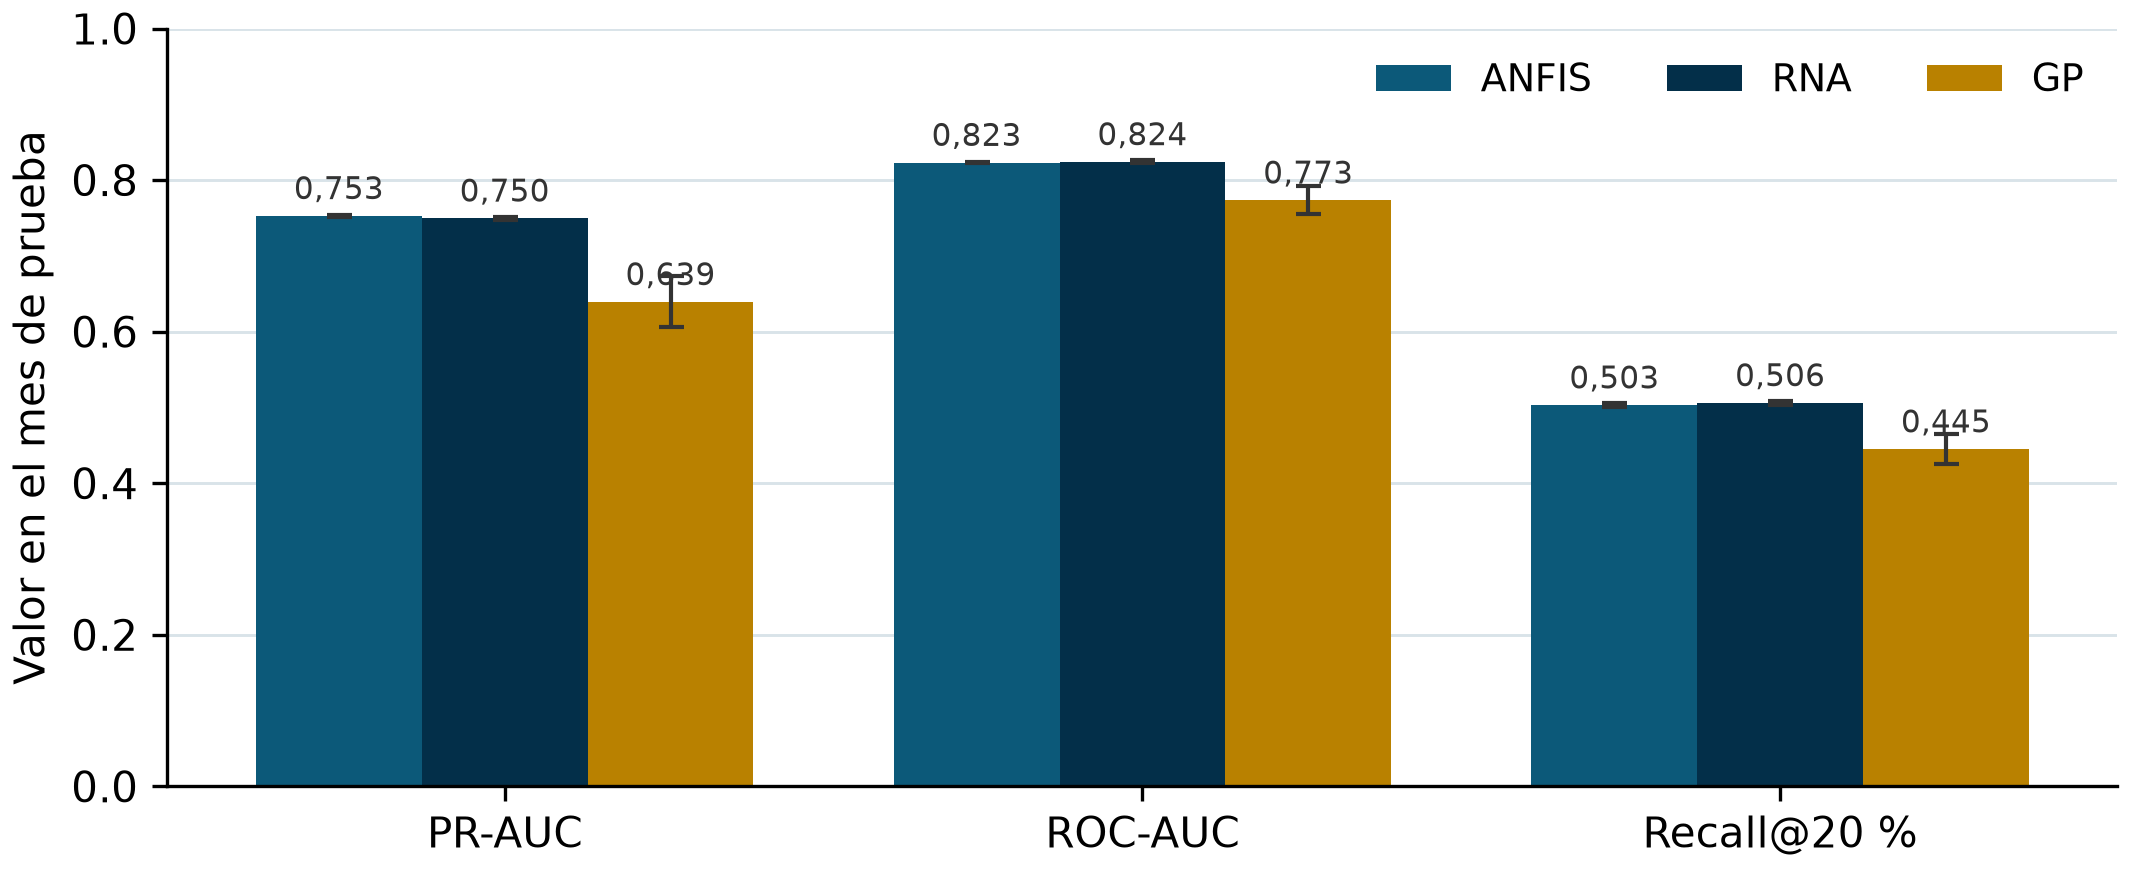
\includegraphics[width=0.72\textwidth]{anfis_rna_gp_comparacion.png}
\caption{Comparación en el conjunto de prueba, por artículo: media y
desviación estándar sobre cinco semillas del ANFIS, la RNA y el GP sobre el
mismo mes de prueba. Las barras de error del ANFIS y la RNA son menores que
el grosor de la línea.}
\label{fig:comparacion}
\end{figure*}

\begin{figure*}[htbp]
\centering
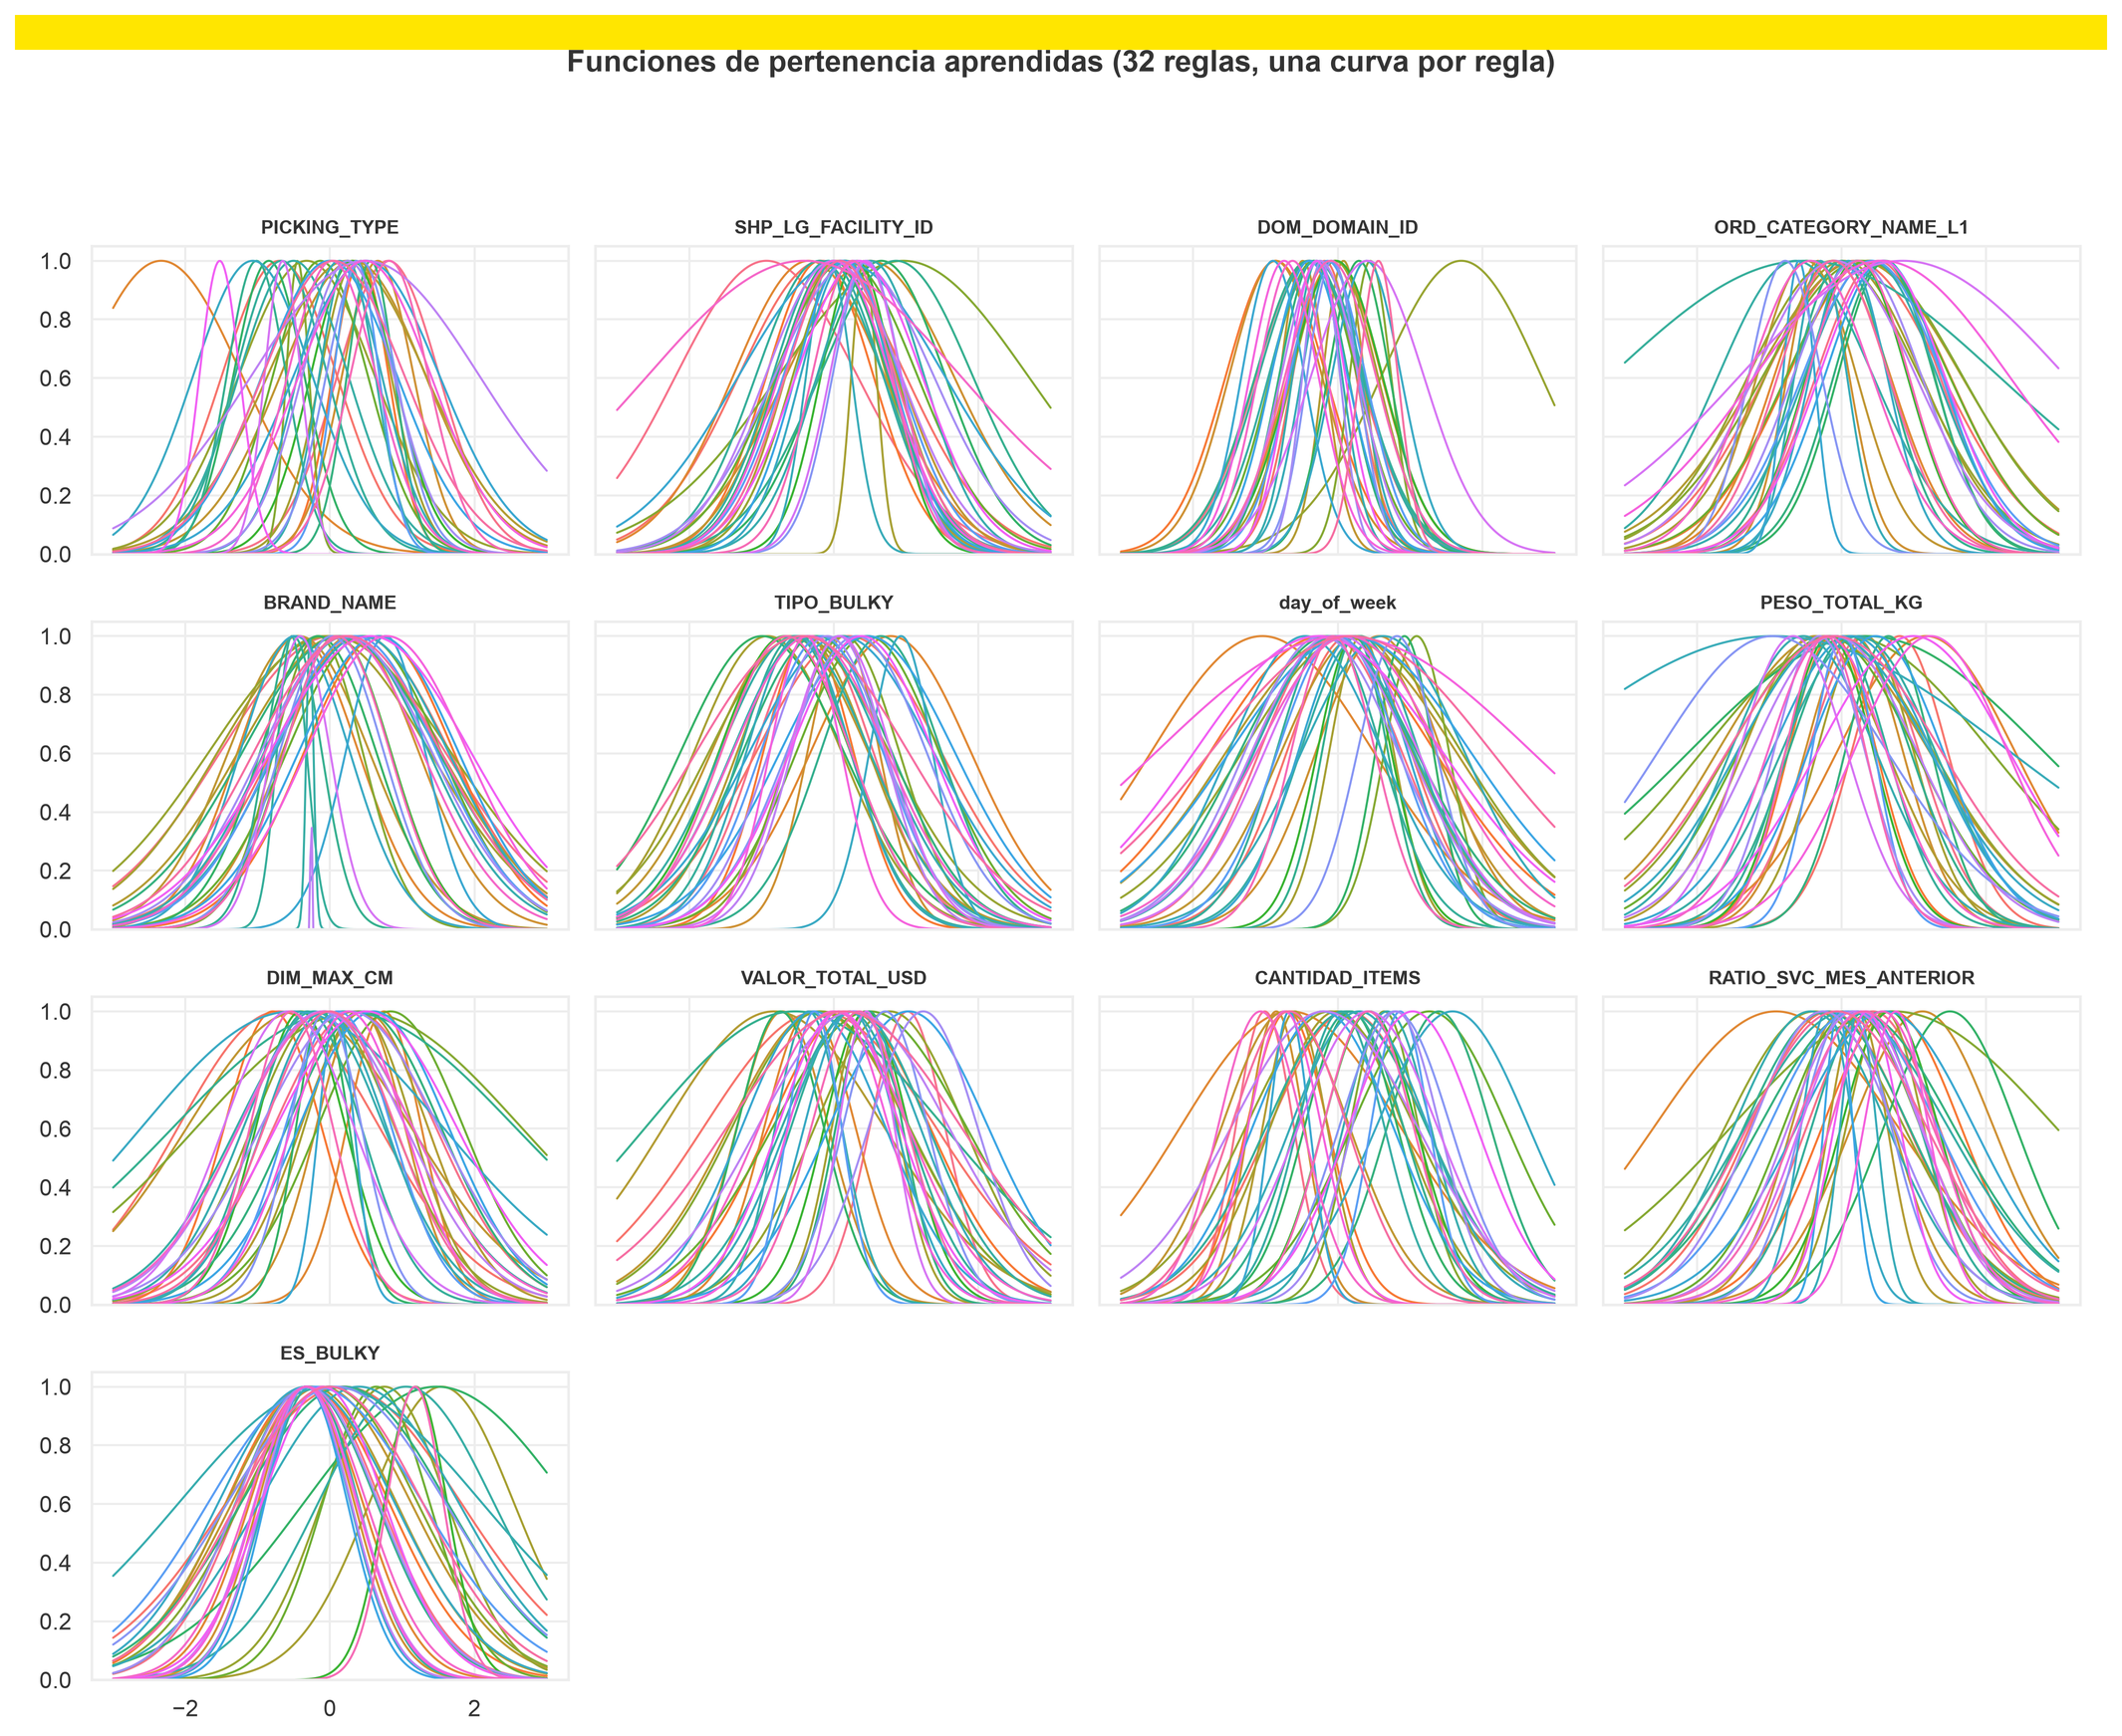
\includegraphics[width=0.92\textwidth]{anfis_funciones_pertenencia.png}
\caption{Funciones de pertenencia gaussianas aprendidas por el modelo de
referencia (semilla 44, 32 reglas, una curva por regla) para cada variable,
en la escala estandarizada de entrenamiento (0 es la media, $\pm1$ una
desviación). Las categóricas aparecen ya codificadas por su tasa de pérdida
(\ref{eq:te}), de modo que ``alto'' en una de ellas significa ``categoría
con alta tasa histórica'', no una categoría concreta.}
\label{fig:pertenencia}
\end{figure*}

\begin{figure}[htbp]
\centering
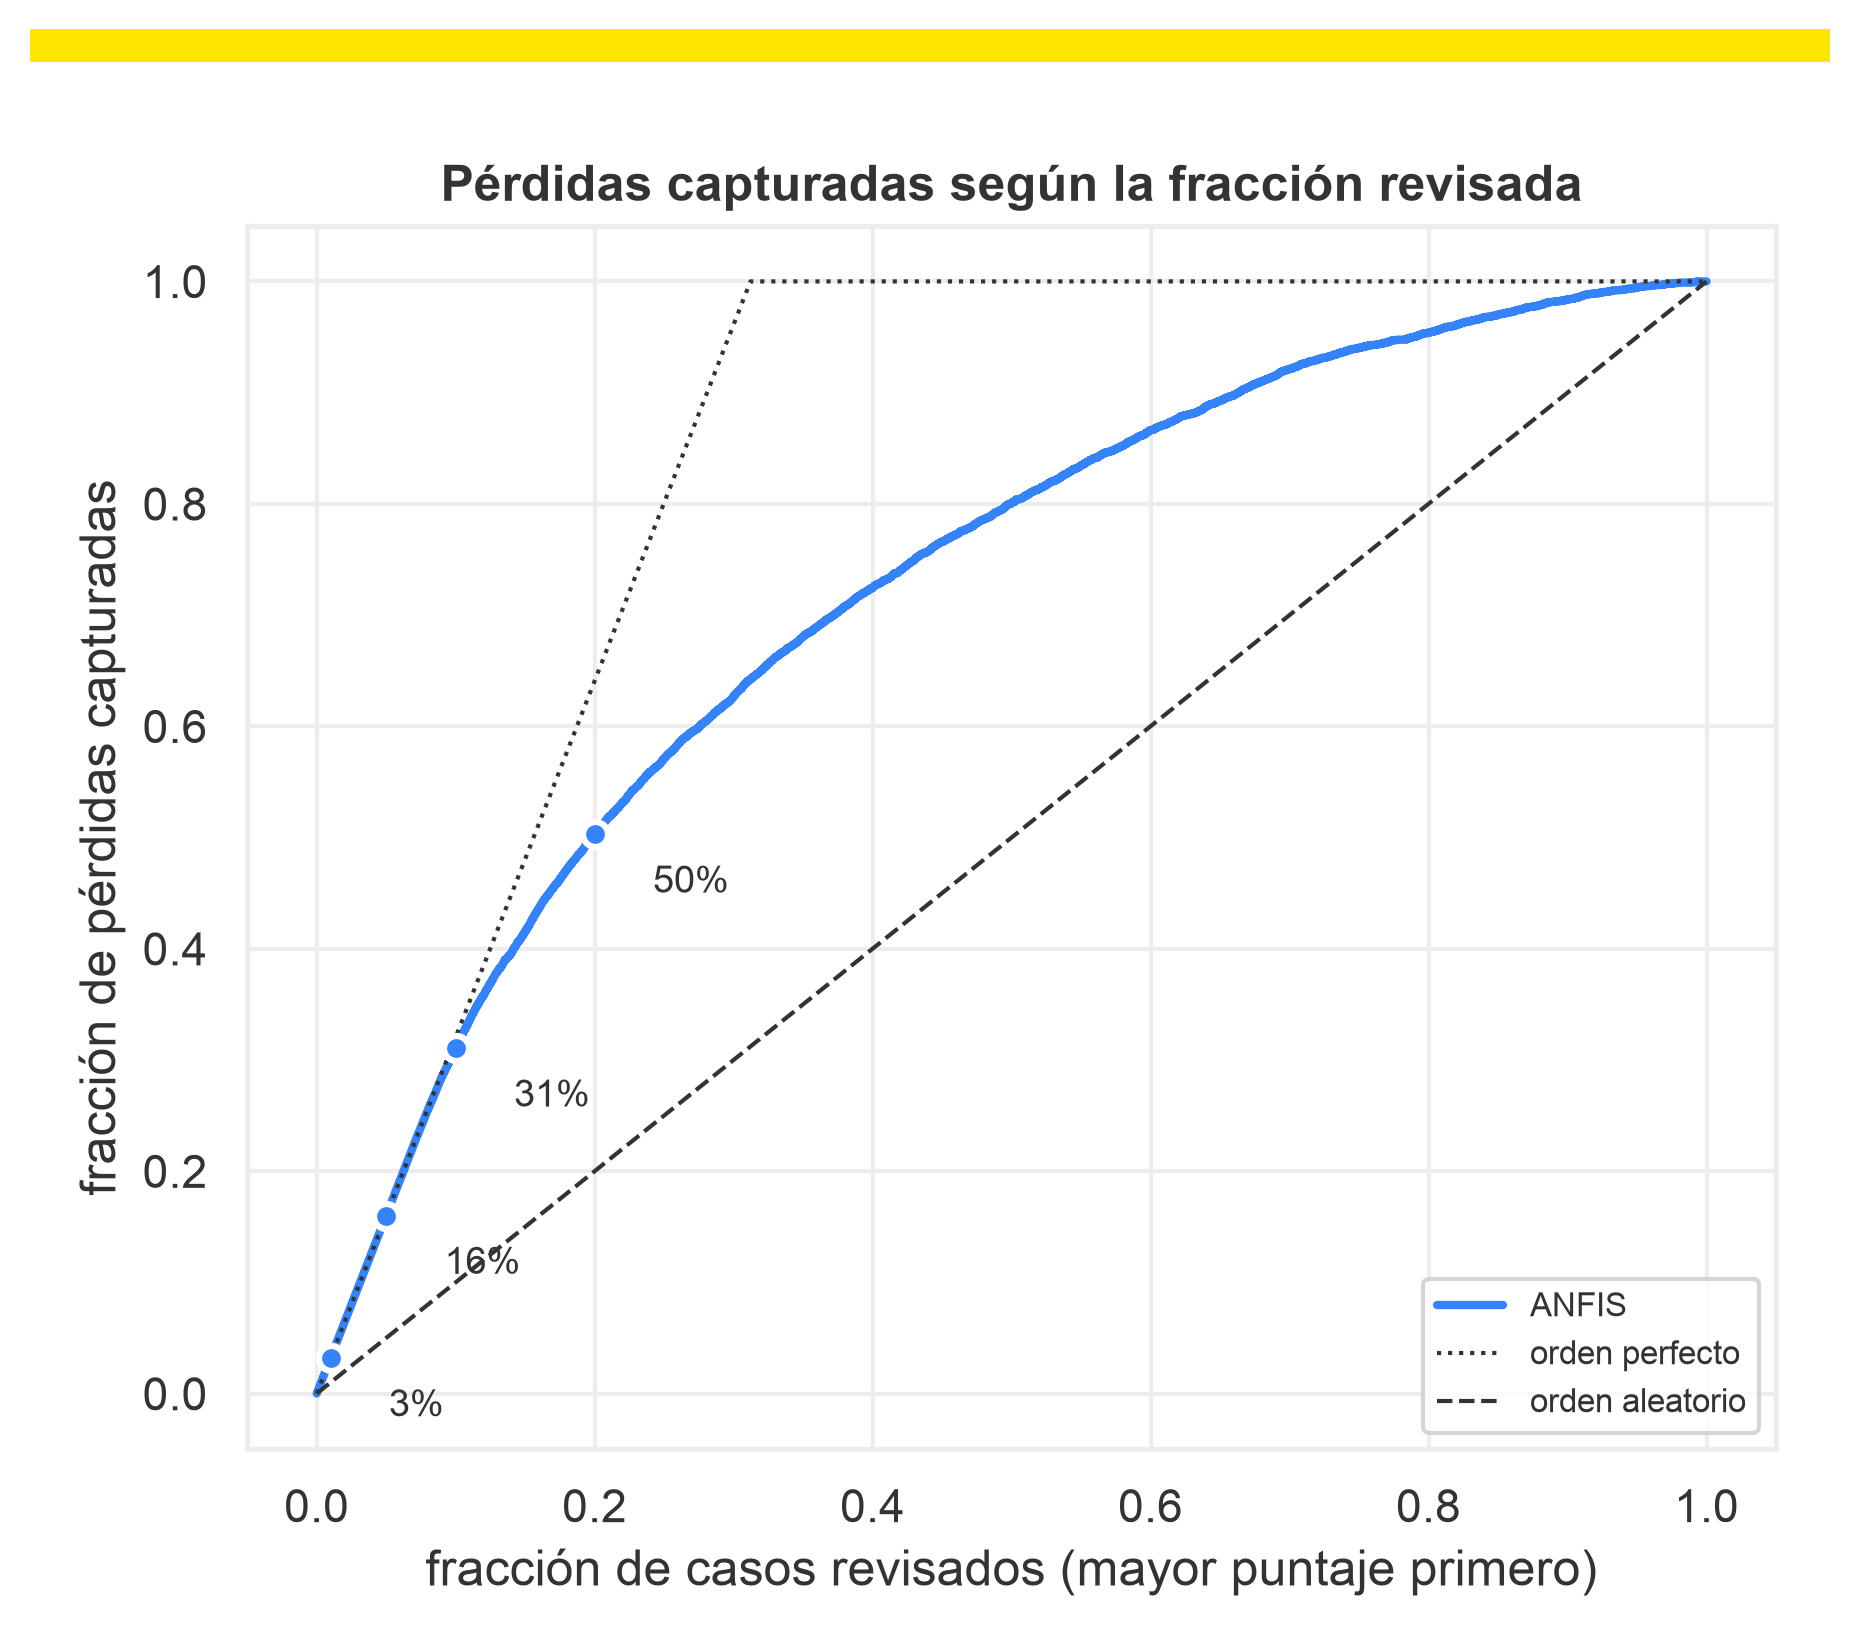
\includegraphics[width=\linewidth]{anfis_curva_ganancia.png}
\caption{Pérdidas capturadas según la fracción revisada para el modelo de
referencia en el mes de prueba. El orden perfecto está acotado por la tasa de
positivos de la muestra (0,312).}
\label{fig:ganancia}
\end{figure}

\begin{figure}[htbp]
\centering
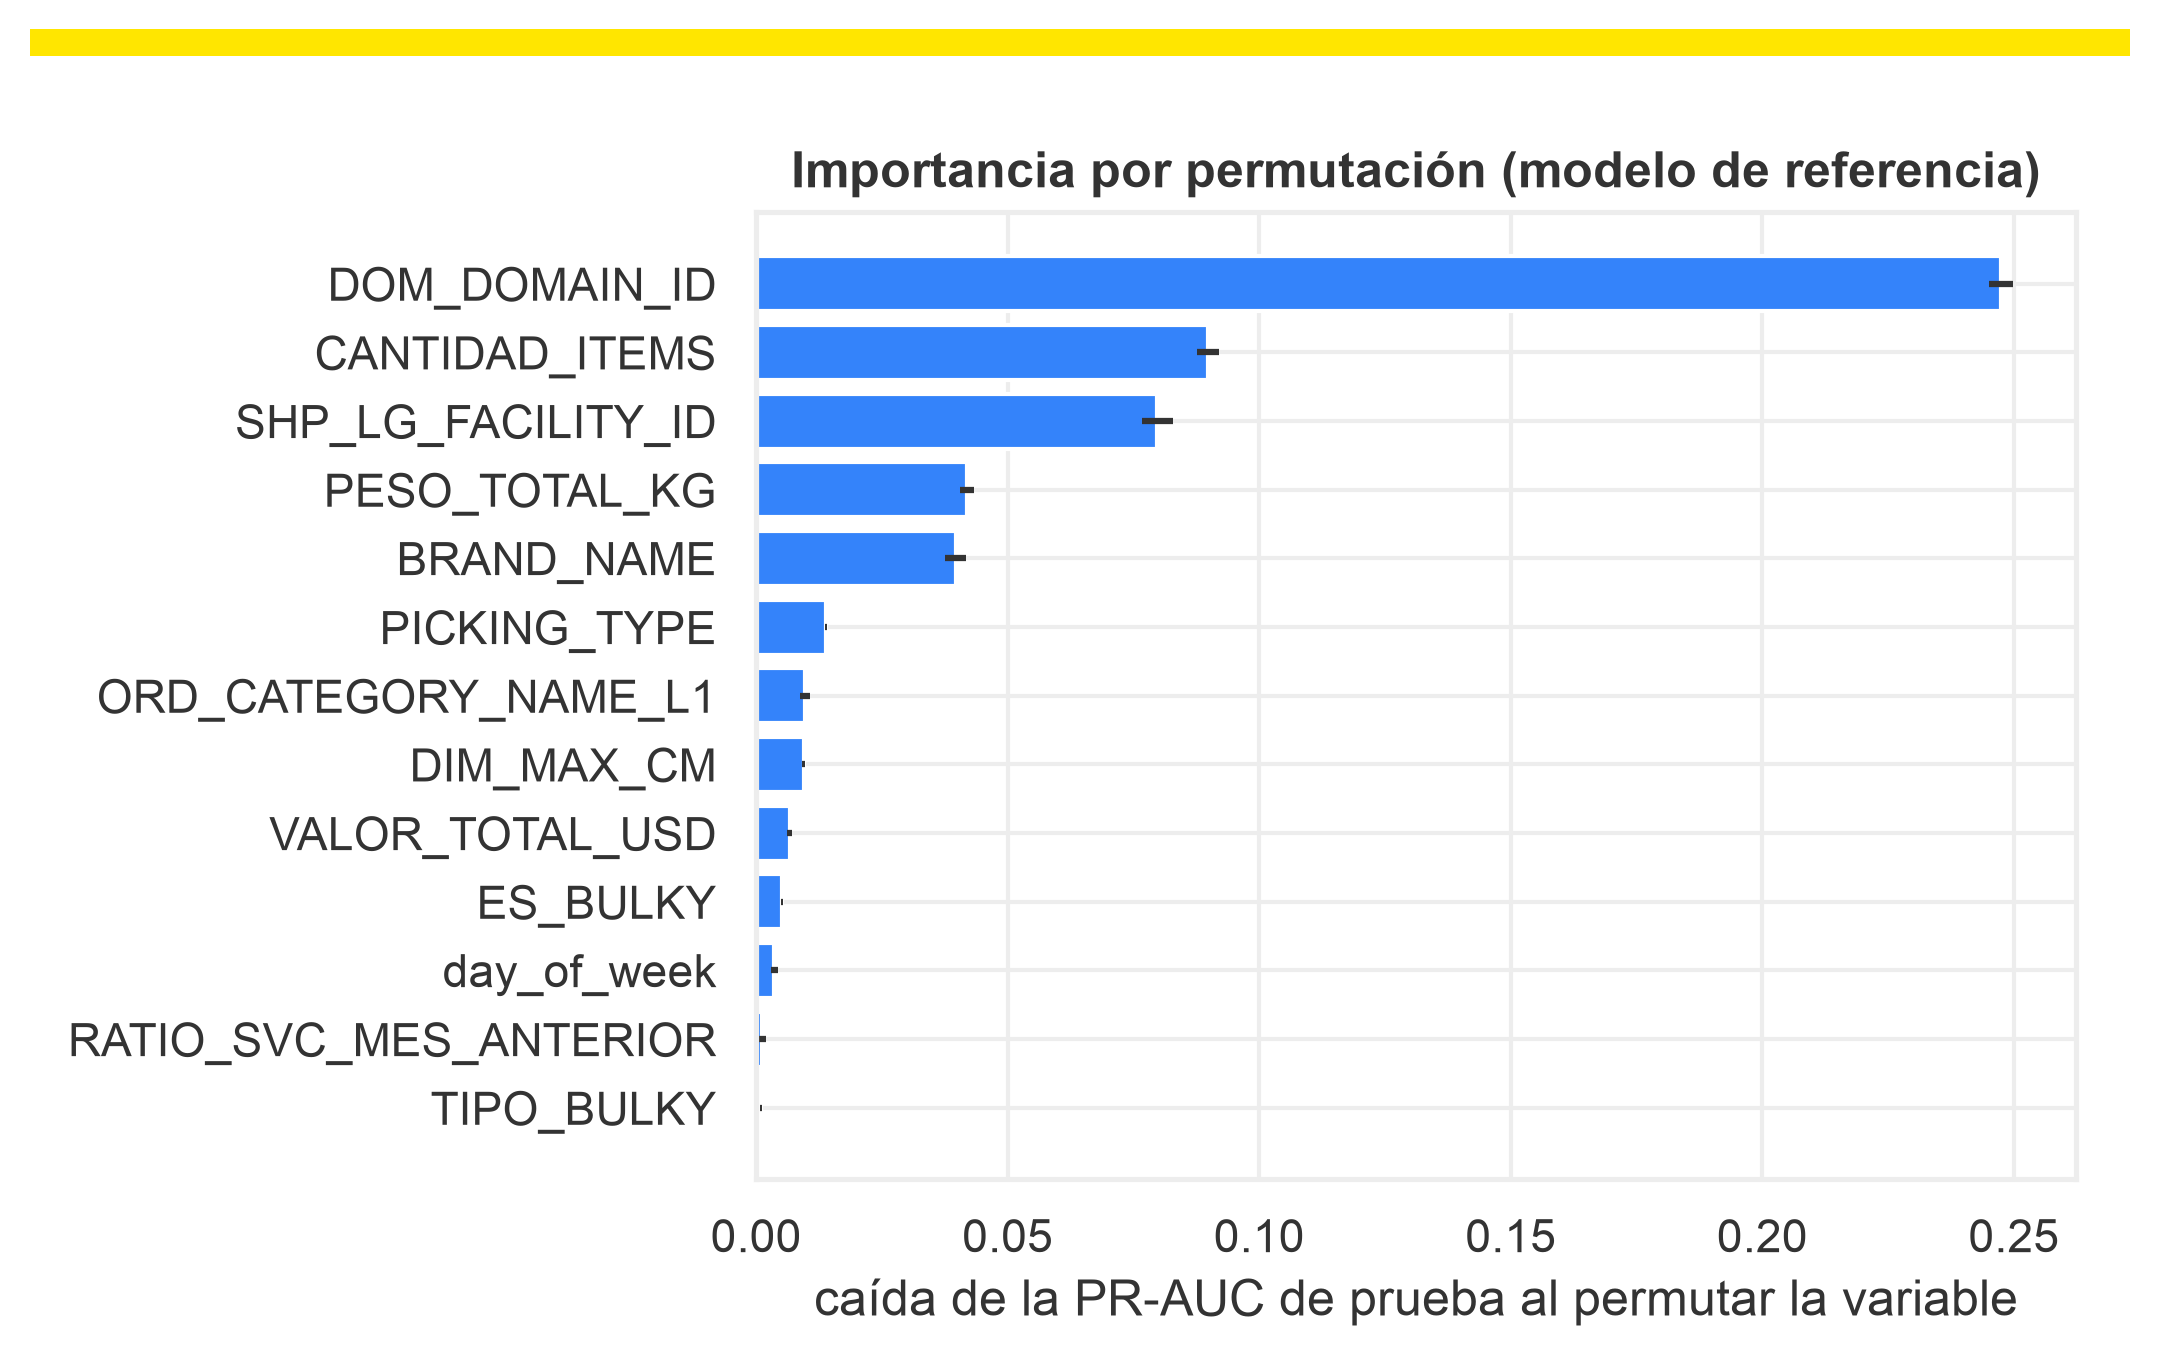
\includegraphics[width=\linewidth]{anfis_importancia_permutacion.png}
\caption{Importancia por permutación del modelo de referencia: caída de la
PR-AUC de prueba al barajar cada variable (media y desviación sobre tres
permutaciones). Mide dependencia, no causalidad.}
\label{fig:importancia}
\end{figure}

\section{Impactos éticos y sociales}

\textbf{Correlación, no causalidad.} Las variables de mayor peso son tasas
históricas de pérdida por dominio, instalación y marca. Un puntaje alto no
indica que la instalación o el vendedor sean responsables; refleja el
historial agregado de una categoría. Que la regla dominante de un envío se
describa como ``dominio de alta tasa, instalación de tasa media'' puede
leerse, erróneamente, como un juicio sobre ese dominio o esa instalación. El
agente se plantea como apoyo a la priorización humana y nunca como mecanismo
automático de sanción a instalaciones, vendedores o transportistas.

\textbf{Sesgo heredado y artefactos de extracción.} Si la base histórica
contiene artefactos, el modelo los reproduce con apariencia de evidencia. El
caso de \col{LG_REGION} ya demostró que una taxonomía puede codificar la
etiqueta; la sospecha equivalente sobre \col{DOM_DOMAIN_ID} (seis valores con
100\,\% de pérdida y 200 a 834 filas cada uno) explica con toda probabilidad
la Precision@1\,\% y @5\,\% perfectas y la tasa de falsos positivos nula en
esos umbrales: la codificación por tasa (\ref{eq:te}) asigna a esos dominios
un valor cercano a 1 que ninguna otra fila alcanza, y una regla con centro
alto en esa variable los separa sin error. La legibilidad del ANFIS lo hace
visible (la regla 8 y la caída de 0,247 al permutar), pero no lo corrige;
obliga a investigar el artefacto en la fuente antes de operar.

\textbf{Confidencialidad y efecto sobre la revisión.} Las tablas de
codificación contienen instalaciones, dominios y marcas de la empresa; el
\textit{notebook} versionado muestra solo agregados (cardinalidades, rangos
de tasas, etiquetas lingüísticas) y ningún identificador de envío. Además,
una lista priorizada concentra la atención en una fracción de los envíos:
con Recall@20\,\% de 0,503, la mitad de las pérdidas quedaría fuera de una
revisión del 20\,\%, y el puntaje debe complementar, no sustituir, los
controles existentes.

\section{Resultados y criterios de comparación}

\textbf{Desempeño predictivo.} El ANFIS y la RNA empatan: +0,0033 de PR-AUC y
$-$0,0010 de ROC-AUC, diferencias dentro de la dispersión entre semillas. El
GP queda 0,114 y 0,050 por debajo del ANFIS. La mejor semilla del GP (PR-AUC
0,689) no alcanza a la peor del ANFIS (0,752).

\textbf{Calidad de la priorización.} En el 10\,\% superior el ANFIS captura
algo más que la RNA (Recall@10\,\% de 0,311 frente a 0,302) con mayor
precisión (0,970 frente a 0,942); en el 20\,\% la RNA recupera la ventaja por
un margen mínimo (0,506 frente a 0,503). Ambas cimas están bajo la misma
sospecha del artefacto de dominio, y la igualdad exacta de Recall@1\,\% en
las dos técnicas (0,0321, el techo) sugiere que ocupan la cima con las mismas
filas.

\textbf{Interpretabilidad.} El ANFIS ofrece una representación intermedia
entre la fórmula del GP y la caja negra de la RNA: 32 reglas, cada una con
13 antecedentes gaussianos graficables y un consecuente lineal, y para cada
envío una regla dominante con su etiqueta lingüística. Esa lectura tiene
límites claros. Con 13 variables por regla, la base no se reduce a reglas
cortas de libro; las categóricas entran ya codificadas, así que ``marca
alta'' significa ``marca de alta tasa histórica''; y las reglas de mayor
cobertura son de riesgo bajo y poco diferenciadas, de modo que la explicación
de un envío de riesgo alto depende de pocas reglas de cola. No se realizó una
evaluación con usuarios que mida comprensión, tiempo de revisión o confianza,
por lo que no se afirma una superioridad empírica en esas dimensiones.

\textbf{Costo computacional.} Unos 5~s por semilla y 1\,280 parámetros,
frente a cerca de 100~s de la RNA y a los 50 a 85~s del GP; sin GPU y sin
AutoGluon. Son medidas de contexto, no un \textit{benchmark} controlado, y
una ventaja de velocidad de este orden solo importaría en reentrenamientos
frecuentes.

\textbf{Estabilidad entre semillas.} El ANFIS es la técnica más estable de
las tres (desviación de PR-AUC de 0,0012, frente a 0,0020 de la RNA y 0,0338
del GP). La inicialización con \textit{fuzzy c-means} y el consecuente
inicializado con la tasa de cada grupo explican en parte esa estabilidad: las
cinco corridas parten de regiones parecidas del espacio de parámetros. Dos
reglas inactivas en el modelo de referencia indican que 32 es un número
holgado; la selección por validación no penalizó esa holgura.

\textbf{Dependencia de \col{DOM_DOMAIN_ID}.} Las tres técnicas dependen del
dominio: caída de 0,247 en el ANFIS y 0,197 en la RNA al permutarlo, y
0,063 en el GP al retirarlo. La magnitud mayor en el ANFIS es coherente con
una codificación que convierte los dominios puros en un valor extremo fácil
de aislar con una gaussiana. La permutación mide dependencia, no causalidad,
y no descarta que otras categóricas conserven una señal correlacionada.

\section{Conclusiones y trabajo futuro}

Un sistema neuro-difuso de tipo Takagi-Sugeno, aprendido de los datos con
información disponible solo al crear el envío y bajo el mismo protocolo
temporal que la red neuronal y el clasificador simbólico, ordena el riesgo de
pérdida al mismo nivel que la RNA (PR-AUC de 0,753~$\pm$~0,001 frente a
0,750~$\pm$~0,002; ROC-AUC de 0,823 frente a 0,824) y muy por encima del GP
(0,639 y 0,773), con la menor dispersión entre semillas de las tres técnicas
y un costo de entrenamiento de segundos. A cambio de la fórmula explícita del
GP, entrega funciones de pertenencia graficables y una base de reglas con
etiquetas lingüísticas y cobertura medida, que hace visible, sin corregirla,
la dependencia del dominio del producto. La respuesta a la pregunta del
módulo es afirmativa en desempeño y matizada en legibilidad: el ANFIS es tan
competitivo como la RNA, y es más legible que ella, pero su base de 32 reglas
sobre 13 variables codificadas no es una explicación de libro.

El resultado metodológico se mantiene: con la limpieza, la partición y las
métricas copiadas literalmente del protocolo de la RNA, la selección del
número de reglas solo en validación y cinco semillas, la comparación entre
técnicas es directa y la igualdad observada es creíble. No prueba
significancia ni generalización a otras cohortes: las desviaciones entre
semillas no son intervalos de confianza poblacionales, y el mes de prueba ya
era conocido. Una evaluación posterior podría estimar la incertidumbre de la
diferencia ANFIS--RNA con remuestreo pareado por envío y probar meses nuevos.

El trabajo futuro inmediato es auditar \col{DOM_DOMAIN_ID} en la fuente,
pues condiciona a las tres técnicas, y repetir el ANFIS sin esa variable como
ablación, igual que se hizo con el GP. Después: agrupar las marcas (por
vendedor o categoría) para reducir el 21\,\% de filas de prueba que hoy
entran con el previo; explorar los hiperparámetros apenas tocados (peso del
previo, ancho mínimo, tasa de aprendizaje, pertenencias de campana
generalizada o triangulares) siempre en validación; podar reglas inactivas o
redundantes y regularizar los anchos para acercar la base a reglas legibles
sin perder orden; y, como cierre del proyecto, evaluar un ensamble que
combine la RNA, el ANFIS y el árbol simbólico con este mismo protocolo.

\IEEEtriggeratref{13}
\begin{thebibliography}{00}
\bibitem{bortolini} M. Bortolini \textit{et al.}, ``A deep learning approach to
predict supply chain delivery delay risk based on macroeconomic indicators: A
case study in the automotive sector,'' \textit{Applied Sciences}, vol. 14,
no. 11, art. 4688, 2024, doi: 10.3390/app14114688.
\bibitem{ye} B. Ye, J. Zuo, X. Zhao y L. Luo, ``Research on the express
delivery delay prediction based on neural network in the background of big
data,'' en \textit{Proc. 6th Int. Conf. Electronic, Mechanical, Information
and Management Society}, 2016, pp. 1449--1454, doi: 10.2991/emim-16.2016.294.
\bibitem{nezamoddini} N. Nezamoddini, A. Gholami y F. Aqlan, ``A risk-based
optimization framework for integrated supply chains using genetic algorithm
and artificial neural networks,'' \textit{Int. J. Production Economics},
art. 107569, 2020, doi: 10.1016/j.ijpe.2019.107569.
\bibitem{ifac2022} D. Wani, R. Singh, V. B. Khanapuri y M. K. Tiwari,
``Delay prediction to mitigate e-commerce supplier
disruptions using voting mechanism,'' \textit{IFAC-PapersOnLine}, vol. 55,
no. 10, pp. 731--736, 2022, doi: 10.1016/j.ifacol.2022.09.495.
\bibitem{gajovic} V. Gajović, M. Kerkez y J. Kočović, ``Modeling and
simulation of logistic processes: Risk assessment with a fuzzy logic
technique,'' \textit{Simulation}, vol. 94, no. 6, 2018,
doi: 10.1177/0037549717738351.
\bibitem{aqlan} F. Aqlan y S. S. Lam, ``A fuzzy-based integrated framework for
supply chain risk assessment,'' \textit{Int. J. Production Economics},
vol. 161, pp. 54--63, 2015, doi: 10.1016/j.ijpe.2014.11.013.
\bibitem{informe_rna} K. Bueno S. y L. Portela L., ``RiskShip: Priorización
inteligente de envíos con riesgo de falla. Solución con redes neuronales,''
informe de proyecto, Pontificia Universidad Javeriana, Bogotá, 2026.
\bibitem{paper_gp} K. Bueno S. y L. Portela L., ``RiskShip: Priorización
inteligente de envíos con riesgo de falla. Solución con programación
genética,'' artículo de proyecto, Pontificia Universidad Javeriana, Bogotá,
2026.
\bibitem{jang} J.-S. R. Jang, ``ANFIS: Adaptive-network-based fuzzy inference
system,'' \textit{IEEE Trans. Syst., Man, Cybern.}, vol. 23, no. 3,
pp. 665--685, 1993, doi: 10.1109/21.256541.
\bibitem{takagi} T. Takagi y M. Sugeno, ``Fuzzy identification of systems and
its applications to modeling and control,'' \textit{IEEE Trans. Syst., Man,
Cybern.}, vol. SMC-15, no. 1, pp. 116--132, 1985,
doi: 10.1109/TSMC.1985.6313399.
\bibitem{zadeh} L. A. Zadeh, ``Fuzzy sets,'' \textit{Information and
Control}, vol. 8, no. 3, pp. 338--353, 1965,
doi: 10.1016/S0019-9958(65)90241-X.
\bibitem{adam} D. P. Kingma y J. Ba, ``Adam: A method for stochastic
optimization,'' en \textit{Proc. 3rd Int. Conf. Learning Representations
(ICLR)}, 2015, doi: 10.48550/arXiv.1412.6980.
\bibitem{guillaume} S. Guillaume, ``Designing fuzzy inference systems from
data: An interpretability-oriented review,'' \textit{IEEE Trans. Fuzzy
Syst.}, vol. 9, no. 3, pp. 426--443, 2001, doi: 10.1109/91.928735.
\bibitem{bezdek} J. C. Bezdek, \textit{Pattern Recognition with Fuzzy
Objective Function Algorithms}. Nueva York, EE.~UU.: Plenum Press, 1981.
\bibitem{fernandez} A. Fernández, S. García, M. J. del Jesus y F. Herrera,
``A study of the behaviour of linguistic fuzzy rule based classification
systems in the framework of imbalanced data-sets,'' \textit{Fuzzy Sets and
Systems}, vol. 159, no. 18, pp. 2378--2398, 2008,
doi: 10.1016/j.fss.2007.12.023.
\bibitem{rudin} C. Rudin, ``Stop explaining black box machine learning models
for high stakes decisions and use interpretable models instead,''
\textit{Nature Machine Intelligence}, vol. 1, no. 5, pp. 206--215, 2019,
doi: 10.1038/s42256-019-0048-x.
\bibitem{micci} D. Micci-Barreca, ``A preprocessing scheme for
high-cardinality categorical attributes in classification and prediction
problems,'' \textit{ACM SIGKDD Explorations Newsletter}, vol. 3, no. 1,
pp. 27--32, 2001, doi: 10.1145/507533.507538.
\bibitem{catboost} L. Prokhorenkova, G. Gusev, A. Vorobev, A. V. Dorogush y
A. Gulin, ``CatBoost: Unbiased boosting with categorical features,'' en
\textit{Advances in Neural Information Processing Systems}, vol. 31, 2018,
doi: 10.48550/arXiv.1706.09516.
\bibitem{deleeuw} J. de Leeuw, Z. Bukhsh y Y. Zhang, ``Parcel loss prediction
in last-mile delivery: Deep and non-deep approaches with insights from
explainable AI,'' preimpresión arXiv:2310.16602, 2023,
doi: 10.48550/arXiv.2310.16602.
\bibitem{zhang2026} Y. Zhang, Y. Wang y Y. Wang, ``A deep tabular learning
framework for e-commerce delivery delay prediction and cost-sensitive
operational risk mitigation,'' \textit{Algorithms}, vol. 19, no. 7, art. 597,
2026, doi: 10.3390/a19070597.
\bibitem{davis} J. Davis y M. Goadrich, ``The relationship between
precision-recall and ROC curves,'' en \textit{Proc. 23rd Int. Conf. Machine
Learning (ICML)}, 2006, pp. 233--240, doi: 10.1145/1143844.1143874.
\bibitem{saito} T. Saito y M. Rehmsmeier, ``The precision-recall plot is more
informative than the ROC plot when evaluating binary classifiers on imbalanced
datasets,'' \textit{PLoS ONE}, vol. 10, no. 3, art. e0118432, 2015.
\bibitem{kaufman} S. Kaufman, S. Rosset, C. Perlich y O. Stitelman, ``Leakage
in data mining: Formulation, detection, and avoidance,'' \textit{ACM Trans.
Knowl. Discov. Data}, vol. 6, no. 4, art. 15, pp. 1--21, 2012,
doi: 10.1145/2382577.2382579.
\bibitem{pytorch} A. Paszke \textit{et al.}, ``PyTorch: An imperative style,
high-performance deep learning library,'' en \textit{Advances in Neural
Information Processing Systems}, vol. 32, 2019,
doi: 10.48550/arXiv.1912.01703.
\end{thebibliography}

\end{document}
